\section{Constructing an effective model}

\co{We consider scenarios for which perturbation theory is useful.}
We illustrate the construction of effective models by considering several representative examples.
The simplest application of effective models is the reduction of finite symbolic Hamiltonians, which appear in the derivation of low-energy dispersions of materials.
Starting from a tight-binding model, one performs Taylor expansions of the Hamiltonian near a $k$-point, and then eliminates several high-energy states~\cite{Luttinger_1955,McCann_2013}.
In the study of superconducting qubits, for example, the Hamiltonian contains several bosonic operators, so its Hilbert space is infinite-dimensional, and the coupling between bosons makes the Hamiltonian impossible to diagonalize.
The effective qubit model describes the analytical dependence of qubit frequencies and couplings on the circuit parameters~\cite{Blais_2004,Zhu_2013,Krantz_2019,Li_2020,Blais_2021,Sete_2021}.
This allows to design circuits that realize a desired qubit Hamiltonian, as well as ways to understand and predict qubit dynamics, for which computational tools are being actively developed~\cite{Groszkowski_2021,Chitta_2022,Li_2022}.
Finally, mesoscopic quantum devices are described by a single particle tight-binding model with short range hoppings.
This produces a numerical Hamiltonian that is both big and sparse, which allows to compute a few of its states but not the full spectrum~\cite{Melo_2023}.
Because only the low-energy states contribute to observable properties, deriving how they couple enables a more efficient simulation of the system's behavior.

\co{We demonstrate how Pymablock solves these problems.}
Pymablock treats all the problems, including the ones above, using a unified approach that only requires three steps:
%
\begin{itemize}
\item Define a Hamiltonian
\item Call \mintinline{python}|pymablock.block_diagonalize|
\item Request the desired order of the effective Hamiltonian
\end{itemize}
%
The following code snippet shows how to use Pymablock to compute the fourth order correction to an effective Hamiltonian $\tilde{\mathcal{H}}$:
%
\begin{minted}{python}
# Define perturbation theory
H_tilde, *_ = block_diagonalize([H_0, H_1], subspace_eigenvectors=[vecs_A, vecs_B])

# Request 4th order correction to the effective Hamiltonian
H_AA_4 = H_tilde[0, 0, 4]
\end{minted}
%
The function \mintinline{python}|block_diagonalize| interprets the Hamiltonian $H_0 + H_1$ as a series with two terms, zeroth and first order and calls the block diagonalization routine.
The subspaces to decouple are spanned by the eigenvectors \mintinline{python}|vecs_A| and \mintinline{python}|vecs_B| of $H_0$.
This is the main function of Pymablock, and it is the only one that the user ever needs to call.
Its first output is a multivariate series whose terms are different blocks and orders of the transformed Hamiltonian.
Calling \mintinline{python}|block_diagonalize| only defines the computational problem, whereas querying the elements of \mintinline{python}|H_tilde| does the actual calculation of the desired order.
This interface treats arbitrary formats of Hamiltonians and system descriptions on the same footing and supports both numerical and symbolic computations.

\subsection{k.p model of bilayer graphene}
\label{sec:bilayer_graphene}

\co{We use bilayer graphene to illustrate how to use Pymablock with analytic models.}
To illustrate how to use Pymablock with analytic models, we consider two layers of graphene stacked on top of each other, as shown in Fig.~\ref{fig:bilayer}.
Our goal is to find the low-energy model near the $\mathbf{K}$ point~\cite{McCann_2013}.
To do this, we first construct the tight-binding model Hamiltonian of bilayer graphene.
%
\begin{figure}[!htbp]
\centering
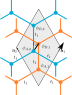
\includegraphics[width=0.3125\linewidth]{figures/bilayer.pdf}
\caption[]{Crystal structure and hoppings of AB-stacked bilayer graphene.}
\label{fig:bilayer}
\end{figure}
%
The main features of the model are its 4-atom unit cell spanned by vectors $\mathbf{a}_1 = (1/2, \sqrt{3}/2)$ and $\mathbf{a}_2=( -1/2, \sqrt{3}/2)$, and with wave functions $\phi_{A,1}, \phi_{B,1}, \phi_{A,2}, \phi_{B,2}$, where $A$ and $B$ indices are the two sublattices, and $1,2$ are the layers.
The model has hoppings $t_1$ and $t_2$ within and between the layers, respectively, as shown in Fig.~\ref{fig:bilayer}.
We also include a layer-dependent onsite potential $\pm m$.

\co{We use sympy.}
We define the Bloch Hamiltonian using the Sympy package for symbolic Python \cite{Meurer_2017}.
%
\begin{minted}{python}
t_1, t_2, m = sympy.symbols("t_1 t_2 m", real=True)
alpha = sympy.symbols(r"\alpha")

H = Matrix([
    [m, t_1 * alpha, 0, 0],
    [t_1 * alpha.conjugate(), m, t_2, 0],
    [0, t_2, -m, t_1 * alpha],
    [0, 0, t_1 * alpha.conjugate(), -m]]
)
\end{minted}
%
$$
H =
\begin{pmatrix}
m & t_1 \alpha & 0 & 0\\
t_1 \alpha^{*} & m & t_2 & 0\\
0 & t_2 & -m & t_1 \alpha\\
0 & 0 & t_1 \alpha^{*} & -m
\end{pmatrix}
$$
%
where $\alpha(\mathbf{k}) = 1 + e^{i \mathbf{k} \cdot \mathbf{a}_1} + e^{\mathbf{k} \cdot \mathbf{a}_2}$, with $k$ the wave vector.
We consider $\mathbf{K}=(4\pi/3, 0)$ the reference point point in $\mathbf{k}$-space: $\mathbf{k} = (4\pi/3 + k_x, k_y)$ because $\alpha(\mathbf{K}) = 0$, making $k_x$ and $k_y$ small perturbations.
Additionally, we consider $m \ll t_2$ a perturbative parameter.

\co{We define the perturbative series.}
To call \mintinline{python}|block_diagonalize|, we need to define the subspaces for the block diagonalization, so we compute the eigenvectors of the unperturbed Hamiltonian at the $\mathbf{K}$ point, $H(\alpha(\mathbf{K}) = m = 0)$.
Then, we substitute $\alpha(\mathbf{k})$ into the Hamiltonian, and call the block diagonalization routine using that $k_x$, $k_y$, and $m$ are perturbative parameters via the \mintinline{Python}|symbols| argument.
%
\begin{minted}{python}
vecs = H.subs({alpha: 0, m: 0}).diagonalize(normalize=True)[0]

H_tilde, U, U_adjoint = block_diagonalize(
    H.subs({alpha: alpha_k}),
    symbols=(k_x, k_y, m),
    subspace_eigenvectors=[vecs[:, :2], vecs[:, 2:]] # AA, BB
)
\end{minted}
%
The order of the variables in the perturbative series will be that of \mintinline{python}{symbols}.
For example, requesting the term $\propto k_x^{i} k_y^{j} m^{l}$ from the effective model is done by calling \mintinline{python}|H_tilde[0, 0, i, j, l]|, where the first two indices are the block indices (AA).
The series of the unitary transformation $U$ and $U^\dagger$ are also defined, and we may use them to transform other operators.

\co{We obtain the effective Hamiltonian.}
We collect corrections up to third order in momentum to compute the standard quadratic dispersion of bilayer graphene and trigonal warping.
We query these terms from \mintinline{Python}|H_tilde| and those proportional to mass to obtain the effective Hamiltonian (shown as produced by the code)\footnote{The full code is available at \url{https://pymablock.readthedocs.io/en/v2.0.0/tutorial/bilayer_graphene.html}.}:
%
{\small
\begin{gather}
\tilde{H}_{\textrm{eff}} =
\begin{bmatrix}
m & \frac{3 t_1^2}{4 t_2} ( - k_x^2 - 2ik_x k_y + k_y^2) \\
\frac{3 t_1^2}{4 t_2} ( - k_x^2 + 2ik_x k_y + k_y^2) & -m
\end{bmatrix} + \nonumber \\
\begin{bmatrix}
\frac{3 m t_1^2}{2 t_2^2} ( - k_x^2 - k_y^2) & \frac{\sqrt{3} t_1^2}{8 t_2} (k_x^3 - 5ik_x^2 k_y + 9 k_x k_y^2 + 3ik_y^3) \\
\frac{\sqrt{3} t_1^2}{8 t_2} (k_x^3 + 5ik_x^2 k_y + 9 k_x k_y^2 - 3ik_y^3) & \frac{3 m t_1^2}{2 t_2^2} (k_x^2 + k_y^2)
\end{bmatrix} \nonumber
\end{gather}
}
%
The first term is the standard quadratic dispersion of gapped bilayer graphene.
The second term contains trigonal warping and the coupling between the gap and momentum.
All the terms take less than two seconds in a personal computer to compute.

\subsection{Dispersive shift of a transmon qubit coupled to a resonator}
\label{sec:cqed}

\co{We illustrate the potential of Pymablock as a useful tool for the design and control of superconducting qubits.}
The need for analytical effective Hamiltonians often arises in circuit quantum electrodynamics (cQED) problems, which we illustrate by studying a transmon qubit coupled to a resonator~\cite{Krantz_2019}.
Specifically, we choose the standard problem of finding the frequency shift of the resonator due to its coupling to the qubit, a phenomenon used to measure the qubit's state~\cite{Blais_2004}.
The Hamiltonian of the system is given by
%
\begin{equation}
    \label{eq:H_cqed}
    \mathcal{H} =
    -\omega_t (a^{\dagger}_{t} a_{t} - \frac{1}{2})
    + \frac{\alpha}{2} a^{\dagger}_{t} a^{\dagger}_{t} a_{t} a_{t} +
    \omega_r (a^{\dagger}_{r} a_{r} + \frac{1}{2}) -
    g (a^{\dagger}_{t} - a_{t}) (a^{\dagger}_{r} - a_{r}),
\end{equation}
%
where $a_t$ and $a_r$ are bosonic annihilation operators of the transmon and resonator, respectively, and $\omega_t$ and $\omega_r$ are their frequencies.
The transmon has an anharmonicity $\alpha$, so that its energy levels are not equally spaced.
In presence of both the coupling $g$ between the transmon and the resonator and the anharmonicity, this Hamiltonian admits no analytical solution.
We therefore treat $g$ as a perturbative parameter.

\co{We truncate the Hamiltonian.}
To deal with the infinite dimensional Hilbert space, we observe that the perturbation only changes the occupation numbers of the transmon and the resonator by $\pm 1$.
Therefore computing $n$-th order corrections to the $n_0$-th state allows to disregard states with any occupation numbers larger than $n_0 + n/2$.
We want to compute the second order correction to the levels with occupation numbers of either the transmon or the resonator being $0$ and $1$.
We accordingly truncate the Hilbert space to the lowest 3 levels of the transmon and the resonator.
The resulting Hamiltonian is a $9 \times 9$ matrix that we construct using Sympy~\cite{Meurer_2017}.

\co{We call block diagonalize and compute the qubit Hamiltonian}
Finally, to compute the energy corrections of the lowest levels, we call \mintinline{python}|block_diagonalize| for each state separately, replicating a regular perturbation theory calculation for single wavefunctions.
To do this, we observe that $H_0$ is diagonal, and use \mintinline{python}|subspace_indices| to assign the elements of its eigenbasis to the $A$ (0) or $B$ (1) subspace.
For example, to find the qubit-dependent frequency shift of the resonator, $\chi$, we start by computing the second order correction to $\ket{0_{t}0_{r}}$:
%
\begin{minted}{python}
indices = [0, 1, 1, 1, 1, 1, 1, 1, 1] # 00 is the first state in the basis
H_tilde, *_ = block_diagonalize(H, subspace_indices=indices, symbols=[g])
H_tilde[0, 0, 2][0, 0] # 2nd order correction
\end{minted}
%
\begin{equation}
    E^{(2)}_{00} = \frac{g^{2}}{-\omega_{r} + \omega_{t}}.
\end{equation}
%
Repeating this process for the other levels requires changing \mintinline{python}|subspace_indices| according to the basis of $H$, and yields the desired resonator frequency shift:
%
\begin{equation}
\begin{aligned}
    \chi &= (E^{(2)}_{11} - E^{(2)}_{10}) - (E^{(2)}_{01} - E^{(2)}_{00}) \\
    & = - \frac{2g^{2}}{\alpha + \omega_{r} - \omega_{t}} + \frac{2g^{2}}{- \alpha + \omega_{r} + \omega_{t}} - \frac{2g^{2}}{\omega_{r} + \omega_{t}} + \frac{2g^{2}}{\omega_{r} - \omega_{t}} \\
    & = - \frac{4 \alpha g^{2} \left(\alpha \omega_{t} - \omega_{r}^{2} - \omega_{t}^{2}\right)}{\left(\omega_{r} - \omega_{t}\right) \left(\omega_{r} + \omega_{t}\right) \left(- \alpha + \omega_{r} + \omega_{t}\right) \left(\alpha + \omega_{r} - \omega_{t}\right)}.
\end{aligned}
\end{equation}
%
In this example, we have not used the rotating wave approximation, including the frequently omitted counter-rotating terms $\sim a_{r} a_{t}$ to illustrate the extensibility of Pymablock.
Computing higher order corrections to the qubit frequency only requires increasing the size of the truncated Hilbert space and requesting \mintinline{python}|H_tilde[0, 0, n]| to the desired order $n$.

\subsection{Induced gap in a double quantum dot}
\label{sec:induced_gap}

\co{Large systems pose an additional challenge due to the scaling of linear
algebra routines for large matrices.}
Large systems pose an additional challenge due to the cubic scaling of linear algebra routines with matrix size.
To overcome this, Pymablock is equipped with an implicit method, which utilizes the sparsity of the input and avoids the construction of the full transformed Hamiltonian.
We illustrate the efficiency of this method by applying it to a system of two quantum dots coupled to a superconductor between them, shown in
Fig.~\ref{fig:QD_spectrum}, and described by the Bogoliubov-de Gennes Hamiltonian:
%
\begin{equation}
    H_{BdG} =
    \begin{cases}
        (\mathbf{k}^2/2m - \mu_{sc}) \sigma_z + \Delta \sigma_x \quad & \text{for } L/3 \leq x \leq 2L/3, \\
        (\mathbf{k}^2/2m - \mu_n) \sigma_z \quad & \text{otherwise},
    \end{cases}
\end{equation}
where the Pauli matrices $\sigma_z$ and $\sigma_x$ act in the electron-hole space, $\mathbf{k}$ is the 2D wave vector, $m$ is the effective mass, and $\Delta$ the superconducting gap.

\co{We use Kwant to build the Hamiltonian of the system.}
We use the Kwant package~\cite{Groth_2014} to build the Hamiltonian of the system~\footnote{The full code is available at \url{https://pymablock.readthedocs.io/en/v2.0.0/tutorial/induced_gap.html}.}, which we define over a square lattice of $L \times W = 200 \times 40$ sites.
On top of this, we consider two perturbations: the barrier strength between the quantum dots and the superconductor, $t_b$, and an asymmetry of the dots' potentials, $\delta \mu$.

The system is large: it is a sparse array of size $63042 \times 63042$, with $333680$ non-zero elements, so even storing all the eigenvectors would take $60$ GB of memory.
The perturbations are also sparse, with $632$, and $126084$ non-zero elements for the barrier strength and the potential asymmetry, respectively.
The sparsity structure of the Hamiltonian and the perturbations is shown in the left panel of Fig.~\ref{fig:QD_spectrum}, where we use a smaller system of $L \times W = 8 \times 2$ for visualization.
Therefore, we use sparse diagonalization~\cite{Virtanen_2020} and compute only four eigenvectors of the unperturbed Hamiltonian closest to zero energy, which are the Andreev states of the quantum dots.
%
\inputminted[firstline=61, lastline=62]{python}{code_figures/lattice_system.py}
%
We now call the block diagonalization routine and provide the computed eigenvectors.
%
\inputminted[firstline=64, lastline=64]{python}{code_figures/lattice_system.py}
%
Because we only provide the low-energy subspace, Pymablock uses the implicit method.
Calling \mintinline{python}|block_diagonalize| is now the most time-consuming step because it requires pre-computing several decompositions of the full Hamiltonian.
It is, however, manageable and it only produces a constant overhead of less than three seconds.

To compute the spectrum, we collect the lowest three orders in each parameter in an appropriately sized tensor.
%
\inputminted[firstline=69, lastline=69]{python}{code_figures/lattice_system.py}
%
This takes two more seconds to run, and we can now compute the low-energy spectrum after rescaling the perturbative corrections by the magnitude of each perturbation.
%
\inputminted[firstline=72, lastline=77]{python}{code_figures/lattice_system.py}
%
Finally, we plot the spectrum of the $2$ Andreev states in Fig.~\ref{fig:QD_spectrum}.
%
\begin{figure}[h!]
\centering
\includegraphics[width=\linewidth]{figures/lattice_system.pdf}
\caption{
    Hamiltonian (left) and Andreev levels (right) of two quantum dots coupled to a superconductor (inset).
    The barrier $t_b$ between the dots and the superconductor, $H_{10}$, and the asymmetry $\delta \mu$ between the dots' potential, $H_{01}$, are perturbations.
}
\label{fig:QD_spectrum}
\end{figure}
%
As expected, the crossing at $E=0$ due to the dot asymmetry is lifted when the dots are coupled to the superconductor.
In addition, we observe how the proximity gap of the dots increases with the coupling strength.

Computing the spectrum of the system for $3$ points in parameter space would require the same time as the total runtime of Pymablock in this example.
This demonstrates the speed of the implicit method and the efficiency of Pymablock's algorithm.
